\documentclass{article}
\usepackage[utf8]{inputenc}
\usepackage{parskip}% http://ctan.org/pkg/parskip
%for degrees
\usepackage{gensymb}
%for bmatrix
\usepackage{amsmath}
% for Sarrus
\usepackage{tikz}
\usetikzlibrary{calc,matrix}

\begin{document}

\section{Algebra}
	\subsection{Exponent Properties}
		\begin{equation}
			\frac{a^n}{a^m} = a^{n-m}
		\end{equation}
		\begin{equation}
			x^a y^a = \left( {xy} \right)^a
		\end{equation}
		\begin{equation}
			x^{\left( {\frac{a}{b}} \right)} = \sqrt[b]{{x^a }}
		\end{equation}
		\begin{equation}
			x^{\left( {a - b} \right)} = \frac{{x^a }}{{x^b }}
		\end{equation}
	\subsection{Properties of radicals}
		\begin{equation}
			\sqrt[n]{a} = a^{\frac{1}{n}}
		\end{equation}
		\begin{equation}
			\sqrt[n]{ab} = \sqrt[n]{a}\sqrt[n]{b}
		\end{equation}
		\begin{equation}
			\sqrt[m]{\sqrt[n]{a}} = \sqrt[nm]{a}
		\end{equation}
		\begin{equation}
			\sqrt[n]{\frac{a}{b}} = \frac{\sqrt[n]{a}}{\sqrt[n]{b}}
		\end{equation}
		\begin{equation}
			\sqrt[n]{a^n} = |a|, \ \ \mbox{if $n$ is even}
		\end{equation}
	\subsection{Complex numbers}
		\begin{equation}
			(a+bi)(c+di) =  ac-bd+(ad+bc)i
		\end{equation}
		\begin{equation}
			(a+bi)(a-bi) =  a^2 + b^2
		\end{equation}
		\begin{equation}
			|a + bi| = \sqrt{a^2+b^2} \ \ \mbox{Complex Modulus}
		\end{equation}
		\begin{equation}
			\overline{(a+bi)}=a-bi
		\end{equation}
	\subsection{Logarithms}	
		\begin{equation}
			\log _b b = 1
		\end{equation}
		\begin{equation}
			\log _b 1 = 0
		\end{equation}
		\begin{equation}
			\log _b (x^r) = r \log _b x
		\end{equation}
		\begin{equation}
			\log _b (xy) = \log _b (x) + \log _b (y)
		\end{equation}
		\begin{equation}
			\log _b \left( \frac{x}{y} \right) = \log _b (x) - \log _b (y)
		\end{equation}
		\begin{equation}
			\log _b \left( x \right) = \log _b \left( c \right)\log _c \left( x \right) = \frac{{\log _c \left( x \right)}}{{\log _c \left( b \right)}}
		\end{equation}
	\subsection{Quadratic Formula}
		\begin{equation}
			x = \frac{{ - b \pm \sqrt {b^2 - 4ac} }}{{2a}} \ \ \mbox{when $ax^2 + bx + c = 0$}
		\end{equation}
\section{Linear Algebra}
	Matrix addition: one by one. (commutative, associative)
	
	Scalar multiplication: all. 

	Matrix "multiplication of rows into columns". Multiplication is not commutative ($AB\neq BA$).
	
	\begin{equation}
		c_{jk} = \sum_{i=1}^{n} a_{ji}b_{ik}
	\end{equation}
	
	Inner or dot product of Vectors
	\begin{equation}
		\langle a,b \rangle = \mathbf{a} \bullet \mathbf{b} = \textbf{a}^T\mathbf{b} 
	\end{equation}

	Matrix to the power $A^0=I$

	Inverse: 
	\begin{equation}
		\begin{bmatrix}
			a & b \\ c & d \\ 
		\end{bmatrix}^{-1} =
		\frac{1}{\det(\mathbf{A})} 
		\begin{bmatrix}
			\,\,\,d & \!\!-b \\ -c & \,a \\ 
		\end{bmatrix} =
		\frac{1}{ad - bc} 
		\begin{bmatrix}
			\,\,\,d & \!\!-b \\ -c & \,a \\ 
		\end{bmatrix}
	\end{equation}
	Identities
	\begin{equation}
		(AB)^T = B^TA^T
	\end{equation}
	\begin{equation}
		(A+B)^T = A^T+B^T
	\end{equation}
	\begin{equation}
		(AB)^{-1} = B^{-1}+A^{-1}
	\end{equation}
	\begin{equation}
		A^kB^l = A^{k+l}
	\end{equation}
	Conjungate transpose / adjugate 
	\begin{equation}
		A^* = (\overline{A})^\mathrm{T} = \overline{A^\mathrm{T}}
	\end{equation}
	Determinants
		\begin{equation}
			\det(\mathbf{A}) = \sum_{\sigma \in S_n} \mbox{sgn}(\sigma) \prod_{i=1}^n A_{i,\sigma_i}
		\end{equation}
		For 3$\times$3 matrices (Sarrus rule)
		\begin{equation}
			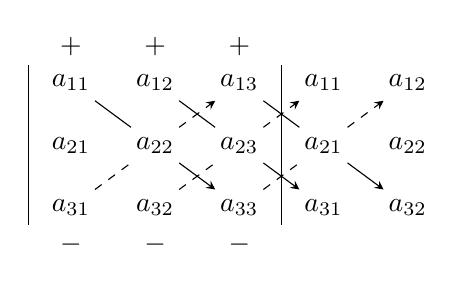
\begin{tikzpicture}[>=stealth]
			\matrix [%
			  matrix of math nodes,
			  column sep=1em,
			  row sep=1em
			] (sarrus) {%
			  a_{11} & a_{12} & a_{13} & a_{11} & a_{12} \\
			  a_{21} & a_{22} & a_{23} & a_{21} & a_{22} \\
			  a_{31} & a_{32} & a_{33} & a_{31} & a_{32} \\
			};

			\path ($(sarrus-1-1.north west)-(0.5em,0)$) edge ($(sarrus-3-1.south west)-(0.5em,0)$)
				  ($(sarrus-1-3.north east)+(0.5em,0)$) edge ($(sarrus-3-3.south east)+(0.5em,0)$)
				  (sarrus-1-1)                          edge            (sarrus-2-2)
				  (sarrus-2-2)                          edge[->]        (sarrus-3-3)
				  (sarrus-1-2)                          edge            (sarrus-2-3)
				  (sarrus-2-3)                          edge[->]        (sarrus-3-4)
				  (sarrus-1-3)                          edge            (sarrus-2-4)
				  (sarrus-2-4)                          edge[->]        (sarrus-3-5)
				  (sarrus-3-1)                          edge[dashed]    (sarrus-2-2)
				  (sarrus-2-2)                          edge[->,dashed] (sarrus-1-3)
				  (sarrus-3-2)                          edge[dashed]    (sarrus-2-3)
				  (sarrus-2-3)                          edge[->,dashed] (sarrus-1-4)
				  (sarrus-3-3)                          edge[dashed]    (sarrus-2-4)
				  (sarrus-2-4)                          edge[->,dashed] (sarrus-1-5);

			\foreach \c in {1,2,3} {\node[anchor=south] at (sarrus-1-\c.north) {$+$};};
			\foreach \c in {1,2,3} {\node[anchor=north] at (sarrus-3-\c.south) {$-$};};
		  \end{tikzpicture}
		\end{equation}
		\begin{equation}
			\det (A \cdot B) = \det (A) \cdot \det (B)
		\end{equation}
		\begin{equation}
			\det (A^{-1}) = \det (A)^{-1}
		\end{equation}
		\begin{equation}
			\det\left(rA\right) = r^n\det(A)\ \ \ \ \mbox{for all $A^{n\times n}$ and scalars $r$}
		\end{equation}
		
		The determinant of a triangular matrix equals the product of the diagonal entries. Since for any triangular matrix A the matrix ${\displaystyle \lambda I-A}$, whose determinant is the characteristic polynomial of A, is also triangular, the diagonal entries of A in fact give the multiset of eigenvalues of A (an eigenvalue with multiplicity m occurs exactly m times as diagonal entry)
		
		
		\subsection{Transpose}
			\begin{equation}
				[A^\mathrm{T}]_{ij} = [A]_{ji}
			\end{equation}
			\begin{equation}
				(A^T)^T = A
			\end{equation}
			\begin{equation}
				(AB)^T = B^TA^T %validated..
			\end{equation}
			\begin{equation}
				det(A^T) = det(A)
			\end{equation}
			\begin{equation}
				(A^T)^{-1} = (A^{-1})^T
			\end{equation}
\section{Trigonometry}
	\subsection{Definitions}
		\begin{equation}
			\sin \theta = \frac{{{\rm{opposite}}}}{{{\rm{hypotenuse}}}}
		\end{equation}
		\begin{equation}
			\tan \theta = \frac{{{\rm{opposite}}}}{{{\rm{adjacent}}}}
		\end{equation}
	\subsection{Standard values}
	\bgroup
	\def\arraystretch{2}
		\begin{table}[hbp]
		\centering
		\begin{tabular}{cccccc}
			\hline
				$\Theta$	& $0\degree$ & $30\degree$ & $45\degree$ & $60\degree$ & $90\degree$ \\  
				$sin \Theta$	& $0$ & $\frac{1}{2}$ & $\frac{1}{\sqrt{2}}$ & $\frac{\sqrt{3}}{2}$ & 1	\\  
				$cos \Theta$	& $1$ & $\frac{\sqrt{3}}{2}$ & $\frac{1}{\sqrt{2}}$ & $\frac{1}{2}$	& 0 \\  
				$tan \Theta$	& $0$ & $\frac{1}{\sqrt{3}}$ & $1$ & $\sqrt{3}$	& / \\  
			\hline
		\end{tabular}
  		\caption{Trigonometric functions standard values}
  		\label{tab:standard-values}
		\end{table}
	\egroup
	\subsection{Formulas and Identities}
		\begin{equation}
			\tan \theta = \frac{\sin \theta}{\cos \theta}
		\end{equation}
		\begin{equation}
			\sin^2 \theta + \cos^2 \theta = 1
		\end{equation}
		
		\begin{equation}
			\sin(-\theta) = - \sin \theta 
		\end{equation}
		\begin{equation}
			\cos(-\theta) = \cos \theta 
		\end{equation}
		
		\begin{equation}
			\sin \left( {\alpha \pm \beta} \right) = \sin \alpha \cos \beta \pm \cos \alpha \sin \beta
		\end{equation}
		\begin{equation}
			\cos \left( {\alpha \pm \beta } \right) = \cos \alpha \cos \beta \mp \sin \alpha \sin \beta
		\end{equation}
		\begin{equation}
			\sin 2\theta = 2\sin \theta \cos \theta
		\end{equation}
		\begin{equation}
			\cos 2\theta = \cos ^2 \theta - \sin ^2 \theta = 2\cos ^2 \theta - 1
		\end{equation}

		\begin{equation}
			\sin ^2 \theta = \frac{1-cos(2\theta)}{2}
		\end{equation}		
		\begin{equation}
			\cos ^2 \theta = \frac{1+sin(2\theta)}{2}
		\end{equation}
		\begin{equation}
			\tan \frac{\theta}{2} = \pm \sqrt{\frac{1-cos(\theta)}{1+cos(\theta)}}
		\end{equation}
		
		Euler's theorem
		\begin{equation}
			e^{ \pm i\theta } = \cos \theta \pm i\sin \theta
		\end{equation}
		\begin{equation}
			\cos \theta = \frac{1}{2} (e^{i\theta} + e^{-i\theta})
		\end{equation}
		\begin{equation}
			\sin \theta = \frac{1}{2i} (e^{i\theta} - e^{-i\theta})
		\end{equation}
\section{Calculus}
	\subsection{Limits}
		\subsubsection{Properties}
			\begin{equation}
				\mathop {\lim }\limits_{x \to a} \left[ cf(x) \right] = c\mathop{\lim }\limits_{x \to a} f(x)
			\end{equation}
			L'Hopital's Rule
			\begin{equation}
				\mathop {\lim }\limits_{x \to c} \frac{{f\left( x \right)}}{{g\left( x \right)}} = \mathop {\lim }\limits_{x \to c} \frac{{f'\left( x \right)}}{{g'\left( x \right)}}
			\end{equation}
		\subsubsection{Evaluations}
			\begin{equation}
				\mathop {\lim }\limits_{x \to 0} \frac{{\sin x}}{x} = 1
			\end{equation}
			\begin{equation}
				\mathop {\lim }\limits_{x \to - \infty } e^x = 0
			\end{equation}
	\subsection{Derivatives}
		\subsubsection{Definition}
			\begin{equation}
				\frac{d}{{dx}}f\left( x \right) = \mathop {\lim }\limits_{h \to 0} \frac{{f\left( {x + h } \right) - f\left( x \right)}}{h }
			\end{equation}
		\subsubsection{Properties}
			\begin{equation}
				\left(fg\right)'=f'g+fg'
			\end{equation}
			Power rule
			\begin{equation}
				\frac{d}{dx}x^n = nx^{n-1}
			\end{equation}
			Chain rule
			\begin{equation}
				\frac{d}{{dx}}\left[ {f\left( u \right)} \right] = \frac{d}{{du}}\left[ {f\left( u \right)} \right]\frac{{du}}{{dx}} \ \ \ \mbox{or} \ \ \ \left(f(g(x)\right)'=f'\left(g(x)\right)g'(x)
			\end{equation}
		\subsubsection{Common Derivatives}
			\begin{equation}
				\frac{d}{{dx}}\left(a^x\right)=a^x\ln(a)
			\end{equation}
			\begin{equation}
				\frac{d}{{dx}}\ln \left( x \right) = \frac{1}{x}, \ \ \ x > 0
			\end{equation}
			\begin{equation}
				\frac{d}{{dx}}\cos x = -\sin x
			\end{equation}
			\begin{equation}
				\frac{d}{{dx}}\sin x = \cos x
			\end{equation}
	\subsection{Integrals}
		\subsubsection{Fundamental Theorem of Calculus}
			\begin{equation}
			\int\limits_a^b {\frac{d}{{dx}}F\left( x \right)dx} = F\left( b \right) - F\left( a \right)
			\end{equation}
		\subsubsection{Properties}
			\begin{equation}
				\int_{}^{}k dx = kx + C
			\end{equation}
		\subsubsection{Common Integrals}
			\begin{equation}
				\int_{}^{}k dx = kx + C
			\end{equation}
			\begin{equation}
				\int_{}^{}x^n dx = \frac{1}{n+1} x^{n+1} + C, \ \ \ \mbox{n $\neq$ -1}
			\end{equation}
			\begin{equation}
				\int_{}^{}\frac{1}{x} dx = \ln|x| + C
			\end{equation}
			\begin{equation}
				\int_{}^{}\ln u = u\ln(u)-u+C
			\end{equation}
			\begin{equation}
				\int_{}^{}e^x dx = e^x+C
			\end{equation}
			\begin{equation}
				\int_{}^{}\sin ax = -\frac{1}{a}\cos ax+C
			\end{equation}
			\begin{equation}
				\int_{}^{}\cos x = \sin x+C
			\end{equation}
			Per partes
			\begin{equation}
				\int {u\frac{{dv}}{{dx}}} dx = uv - \int {\frac{{du}}{{dx}}} vdx
			\end{equation}
			Substitution Rule			
			\begin{equation}
				\int {f(u)\frac{du}{dx}} dx = f(u)du
			\end{equation}
			
	\subsection{Laplace transforms}
		\subsubsection{Definition}
			\begin{equation}
				X(s) = \int\limits_0^\infty {x(t)e^{ - st} dt}
			\end{equation}
		\subsubsection{Properties}
			\begin{equation}
				1 \Leftrightarrow \frac{1}{{s}}
			\end{equation}
			Kroeneker delta function
			\begin{equation}
				\delta (t) \Leftrightarrow 1
			\end{equation}
			\begin{equation}
				Ke^{ - at} u(t) \Leftrightarrow \frac{K}{{s + a}}			
			\end{equation}
			\begin{equation}
				t^n u(t) \Leftrightarrow \frac{{n!}}{{s^{n + 1} }}
			\end{equation}
			\begin{equation}
				\sin (\alpha t)u(t) \Leftrightarrow \frac{\alpha }{{(s^2 + \alpha ^2 )}}
			\end{equation}
			\begin{equation}
				\cos (\alpha t)u(t) \Leftrightarrow \frac{s}{{(s^2 + \alpha ^2 )}}
			\end{equation}
			\begin{equation}
			e^{ - at} \sin (\Omega t)u(t) \Leftrightarrow \frac{\Omega }{{(s + a)^2 + \Omega ^2 }}
			\end{equation}
			\begin{equation}
				e^{ - at} \cos (\Omega t)u(t) \Leftrightarrow \frac{{s + a}}{{(s + a)^2 + \Omega ^2 }}
			\end{equation}

			\begin{equation}
				e^{at} x(t) \Leftrightarrow X(s-a)
			\end{equation}			
			
			Time domain scaling
			\begin{equation}
				x(at)u(t) \Leftrightarrow \frac{1}{a}X\left( {\frac{s}{a}} \right)
			\end{equation}
			Time domain shifting 
			\begin{equation}
				x(t - a)u(t - a) \Leftrightarrow e^{ - as} X(s + a)
			\end{equation}
			Derivative
			\begin{equation}
				\frac{{d^n x(t)}}{{dt^n }} \Leftrightarrow s^n X(s) \ \ or \ \ \mathcal{L}[\dot{x}] = sX(s)-x(0+)
			\end{equation}
			Integral			
			\begin{equation}
				\int{x(t)dt} \Leftrightarrow \frac{X(s)}{s}
			\end{equation}			
			
			Convolution
			\begin{equation}
			\int\limits_0^\infty {x_1 (\tau )x_2 (t - \tau )d\tau } \Leftrightarrow X_1 (s)X_2 (s)
			\end{equation}
\section{Greek letters}

\bgroup
\def\arraystretch{2}
\begin{table}[hbp]
  \centering
  \begin{tabular}{cccc}
  \hline
  	$\alpha A$				& Alpha		& $\nu N$		& Nu	\\
  	$\beta B$				& Beta		& $\xi \Xi$	&  Xi 		\\
  	$\gamma \Gamma$			& Gamma		& $o O$	& Omicron		\\
	$\delta \Delta$			& Delta 	& $\pi \Pi$	& Pi		\\
	$\epsilon \varepsilon $	& Epsilon	& $\rho\varrho P$ & Rho   \\
	$\zeta Z$				& Zeta		& $\sigma \Sigma$& Sigma  	\\
	$\eta H$				& Eta		& $\tau T$	& Tau  		\\  
	$\theta \vartheta \Theta$	& Theta & $\upsilon \Upsilon$ & Upsilon  \\
	$\iota I$				& Iota		& $\phi \varphi \Phi$ & Phi    \\
	$\kappa K$				& Kappa		& $\chi X$	& Chi  		\\
	$\lambda \Lambda$		& Lambda	& $\psi \Psi$	& Psi  	\\
	$\mu M$					& Mu 		& $\omega \Omega$ & Omega   \\
  
  \hline
  \end{tabular}
  \caption{Greek letters}
  \label{tab:symbol-variants}
\end{table}
\egroup


\end{document}